%%%%%%%%%%%%%%%%%%%%%%%%%%%%%%%%%%%%%%%%%%%%%%%%%%%%%%%%%%%%%%%%%%%
%                                                                 %
%   PAW   - Reference Manual -- LaTeX Source                      %
%                                                                 %
%   Chapter 9: Distributed PAW                                    %
%                                                                 %
%   EPS file      : none                                          %
%                                                                 %
%   Editor: Michel Goossens / CN-AS                               %
%   Last Mod.:  8 Feb 1994 20:15 mg                               %
%                                                                 %
%%%%%%%%%%%%%%%%%%%%%%%%%%%%%%%%%%%%%%%%%%%%%%%%%%%%%%%%%%%%%%%%%%%

\chapter{Distributed PAW}
\label{sec:H1DIST}
 
With the increasing number of workstations, it happens more and more
frequently that a user wants to run PAW on a mainframe
or on a workstation.
Several tools described in this chapter have been developed in order to use
in the most convenient way all the resources available in an heteregoneous
environment of workstations, superminis, data acquisition systems
and mainframes.
 
\index{TCP/IP}
\index{DECNET}
\index{OSI}
\index{TELNET}
\index{VAX}
\index{TCPAW}
\begin{DL}{MMMMM}
\item[TELNETG:]A powerful terminal emulator. An alphanumeric window (line mode)
is created on the local workstation (e.g. Apollo)
to create a session (like with \Lit{TELNET})
on a remote computer (e.g. VAX). On the remote computer, a graphics program
is run and a window is automatically created on the local workstation
to receive the graphics output.
\item[3270G
]Same as the \Lit{TELNETG} emulator for the case of a connection
with an IBM machine in full screen mode under VM/CMS.
\item[ZFTP
]The ZEBRA file transfer program optimized to transport ZEBRA
RZ or FZ files between machines with different data representations.
\end{DL}
\index{ZEBRA}
\index{remote!access}
\index{TELNETG}
\index{3270G}
\index{zftp}
 
There exists also the possibility to access files on a {\bf remote computer}
from a PAW session on a workstation.
PAW can be used in a {\bf real time} environment.
Access to HBOOK histograms being filled
\index{global!section}
\index{OS9!module}
by a different process on the same machine (Global sections on VAX) or a
computer on the network (e.g. OS9 modules).
 
Both ZFTP and real time access to histograms on a remote
computer require the implementation of a  {\bf PAW server}
on this computer. The PAW server is automatically started
from a PAW session, if PAW has been implemented with
the relevant options (PATCHY \cite{bib-PATCHY} flag CZ).
PAW and the PAW server must be linked with two special modules
called {\bf CZ} and {\bf TCPAW} \cite{bib-TCPAW1,bib-TCPAW2}.
 
{\bf CZ} is a small FORTRAN package (about 300 lines). It provides
an interface between the ZEBRA Input/Output routines
and the high level transport routines of the TCPAW package.
 
{\bf TCPAW}\cite{bib-TCPAW1}
is a networking package, written in C by Ben Segal (about 1500 lines).
It provides a very simple FORTRAN-callable interface to TCP/IP services.
It supports client and server modules running on UNIX, Apollo, VMS,
VM/CMS and OS9 environments. Small parts of TCPAW
are CERN specific but it would be perfectly possible
to transport it elsewhere with minor modifications. The package
currently requires the Wollongong (TWG) TCP/IP software
to be present on VMS connected systems, the IBM FAL 1.2 Product
on VM/CMS, and Microware TCP/IP on OS9. The UNIX systems
Ultrix, CRAY Unicos, SUN OS, IBM AIX, Apollo/Aegis, Apple A/UX and HP-UX
are supported as delivered.

\section{TELNETG and 3270G}
\index{TELNETG}
\index{3270G}
\index{PAW!server}
\index{CZ}
\index{TCPAW}
 
Figure \ref{fig:FTELNETG}
describes the functionality of these two programs.
They allow
to run a graphics application based on HIGZ (e.g. PAW, GEANT, etc.) on a host
machine and to receive the graphics output on the local machine. TELNETG is
designed to work with operating systems supporting a command line interface
and 3270G for a full screen interface.
 
TELNETG and 3270G supports both graphics Input and Output. The graphics
locator (commands LOCATE, VLOCATE, etc.) as well as the various KUIP graphics menu
styles (G and GP) may be used.
 
Both programs exploit the fact that the HIGZ macro primitives are very
compact, therefore reducing the amount of information to be sent through
the network. Compared to more conventional emulators (4014, 4207, etc.)
gains in speed are typically a factor of 10 when drawing one-dimensional histograms
and may reach a factor 100 for two-dimensional plots (lego, surface, scatterplot).
 
\newpage

\begin{figure}[p]
\epsfig{file=telnetg.eps,height=.9\textheight}
\caption{The TELNETG program}
\label{fig:FTELNETG}
\end{figure}
\clearpage

TELNETG combines a slightly modified version of the standard TELNET
program written in the C language and an interface to the HIGZ system written in FORTRAN.
 
The following example shows how to use TELNETG from an Apollo to a VAX.
The integer identifier of the workstation type  must be preceded by a
{\bf minus sign} (e.g. for an Apollo DN3000):
\begin{XMPt}{Example of a TELNETG session}
$ \Ucom{TELNETG vxcrna}
Trying...
Open
         This is the CERN Central VAXcluster running VMS V5.1

Username: \Ucom{USERNAME}
Password: \Ucom{PASSWORD}(not echoed)
        Welcome to VAX/VMS version V5.1 on node VXCRNA
 TERMINAL TYPE <? for HELP; No default>:\Ucom{D1}
VxCrnA$ \Ucom{PAW}
 ******************************************************
 *                                                    *
 *            W E L C O M E    to   P A W             *
 *                                                    *
 *           Version 1.11/02  29 March 1991           *
 *                                                    *
 ******************************************************
 Workstation type (?=HELP) <CR>=7878 : \Ucom{-10002}
 VERSION 7.4/2.6 OF GKSGRAL STARTED
 PAW > \Ucom{hi/plot 10}           | The graphics is sent to the Apollo
 PAW > \Ucom{locate}               | Graphics input using the Apollo mouse
\end{XMPt}
 
\newpage 
\section{ZFTP}
\label{sec:H2ZFTP}
 
\index{FTP}
\index{ZFTP}
The ZFTP program
(ZEBRA File Transfer Program) provides the same functionality
\index{TELNET}
as the \Lit{FTP} program which is available like \Lit{TELNET} on
all workstations
and mainframes supporting TCP/IP. In addition ZFTP has been optimized
to allow the transfer of ZEBRA binary files both sequential and direct access.
 
\index{ZEBRA!RZ file}
The direct access ZEBRA/RZ files (used for HBOOK histograms and HIGZ pictures)
contain data in the local data representation. Because ZEBRA is an object
oriented language supporting machine independent Input/Output, ZFTP is able
to translate in flight all the ZEBRA data structures in a transparent way
in the network buffers. ZFTP copies the RZ files on the local machine
with the same parameters (RECL, quota, etc.) than on the remote machine.
The original date and time of the objects is also preserved.
 
In addition to binary file transfer, ZFTP can also transfer alphanumeric
text files (up to 80 characters/line). On IBM/VM-CMS, these files must be
of type \Lit{RECFM=F,LRECL=80}.
 
The ZFTP user interface is based on KUIP and is the same on all systems.
If several files have to be transferred (maybe on a regular basis),
KUIP macros may be used. The following commands are available:
\begin{DL}{MMMMM}
\item[OPEN
]To start a communication with a remote machine.
\item[CLOSE
]Close the current communication.
\item[GETA
]Transfer an Alphanumeric text file from the remote machine.
\item[PUTA
]Transfer an Alphanumeric text file to a remote machine.
\item[GETRZ
]Transfer a RZ file from a remote machine.
\item[PUTRZ
]Transfer a RZ file to a remote machine.
\item[GETFZ
]Transfer a FZ file from a remote machine.
\item[PUTFZ
]Transfer a FZ file to a remote machine.
\item[RSHELL
]Send a command to a remote machine.
\end{DL}
\begin{XMPt}{Example of a ZFTP session}
# Start execution of the program from inside the PAW directory
$ \Ucom{ZFTP}
ZFTP > \Ucom{open CERNVM}                       |Starts communication with CERNVM
                                         | (prompt for username/password)
ZFTP > \Ucom{getrz RZFILE.DAT.D  local.dat}     | Transfer IBM file "RZFILE.DAT"
                                         |  to local file "local.dat"
ZFTP > \Ucom{puta local.car}                    | Transfer local alphanumeric file
                                         | "local.car" to IBM
                                         | IBM file name will be "LOCAL CAR A"
ZFTP > \Ucom{quit}
\end{XMPt}
 
\Section{14cm}{Access to remote files from a PAW session}
 
\index{remote!file}
\index{remote!shell}
\index{remote!login}
\index{RSHELL}
\index{RLOGIN}
When running PAW, it is often necessary to access files
(e.g. HBOOK files) which reside on a different computer. 
The ZFTP program described
above can be used if a very frequent access to the file is required. A
more convenient mechanism is the possibility to access the 
files directly. On many systems, one may now use \Lit{NFS}~\cite{bib-NFS}
for this purpose. Under some circumstances, for example if the HBOOK
file is not in exchange mode and it is to be accessed from a computer
running a different operating system, an alternate approach is required.
To fill this gap the PAW server is provided. This works using
a conventional Client/Server model. The client
(PAW) typically runs on a workstation. When the PAW command RLOGIN is invoked,
a PAW server is automatically started on the remote machine, normally
a mainframe or data server. 
 
Once the \Lit{RLOGIN REMOTE} command has been executed, the PAW Current Directory
is set to \Lit{//REMOTE}. The PAW client can now instruct the PAW server to
attach a file using the \Lit{RSHELL} command (e.g. \Lit{rshell file pawtest.dat}). If an
histogram with HBOOK ID=10 is on the remote file, than the PAW command
\Lit{Histo/Plot 10}
will plot this histogram on the local workstation. The histogram resides
on \Lit{//PAWC} like other histograms coming from local files.
 
The \Lit{RSHELL} command may be used to communicate with the PAW server.
The expression typed following \Lit{RSHELL} is passed to the server. The current
implementation of the PAW server recognizes the commands:
\begin{DLtt}{123456789012345678890}
\item[rshell file filename]Server connects filename
\item[rshell cdir //lun11] Server changes current directory
\item[rshell ld]           Server lists current directory
\item[rshell ld //]        Server lists all connected files
\item[rshell message]      Server pass message to operating system
\end{DLtt}
 
\begin{XMPt}{Access to remote files from a workstation}
PAW > \Ucom{rlogin CERNVM}                         | connect to CERNVM
PAW > \Ucom{rshell file HRZTEST.DAT}               | PAW server connects HRZTEST DAT A to //LUN11
PAW > \Ucom{histo/plot 10}                         | plot histogram 10 from CERNVM
PAW > \Ucom{histo/fit 20 G}                        | fit histo 20 with a gaussian and plot it
PAW > \Ucom{rlogin VXCRNA}                         | connect to VXCRNA
PAW > \Ucom{rshell file DISK$DL:[PAW]HEXAM.DAT;3}  | PAW server on VXCRNA connects file to //LUN11
PAW > \Ucom{histo/plot 110}                        | plot histogram 110 from VXCRNA
PAW > \Ucom{rshell file HRZTEST.DAT}               | PAW server on VXCRNA connects file to //LUN12
PAW > \Ucom{histo/plot 110 s}                      | plot histogram 110 from HRZTEST.DAT
                                            | on VXCRNA on the existing picture
PAW > \Ucom{rshell ld //}                          | list all files connected on VXCRNA
PAW > \Ucom{cdir //CERNVM}                         | Change current PAW directory to CERNVM
PAW > \Ucom{histo/plot 110}                        | plot histogram 110 from CERNVM
PAW > \Ucom{histo/plot //VXCRNA/110}               | plot histogram 110 from VXCRNA
PAW > \Ucom{cdir //PAWC}                           | current directory to local memory
PAW > \Ucom{histo/list}                            | list all histograms in //PAWC
PAW > \Ucom{Histo/delete 0}                        | delete all histograms in memory
PAW > \Ucom{hrin //VXCRNA/0}                       | read all histograms from VXCRNA
                                            | file HRZTEST.DAT to //PAWC
PAW > \Ucom{cdir //CERNVM}                         | change directory to CERNVM
PAW > \Ucom{rshell file NEW.DAT.D 1024 N}          | creates a new file on the D disk
PAW > \Ucom{hrout 0}                               | write all histograms from //PAWC
                                            | to CERNVM file NEW DAT D
\end{XMPt}
 
\section{Using PAW as a presenter on VMS systems (global section)}
 
\begin{minipage}{.48\textwidth}
\begin{XMP}
      PROGRAM PRODUCE
      PARAMETER MAXPAGES=100
      COMMON/PAWC/IPAWC(128*MAXPAGES)
      CHARACTER*8 GNAME
      INTEGER*4 HCREATEG
*
      GNAME='GTEST'
      WAIT_TIME=1.
      NUMEVT=1000
*...............           Create Global section
      NPAGES=HCREATEG(GNAME,IPAWC,128*MAXPAGES)
      IF(NPAGES.GT.0) THEN
         PRINT 1000,GNAME
 1000    FORMAT(' Global Section: ',A,' created')
      ELSE
         IERROR=-NPAGES
         PRINT 2000,IERROR
 2000    FORMAT(' Global Section Error', I6)
         GO TO 99
      ENDIF
      CALL HLIMIT(128*NPAGES)
*...............           Book histos.
      CALL HBOOK1(10,'Test1$',50,-4.,4.,0.)
      CALL HBOOK1(20,'Test2$',50,-4.,4.,0.)
*...............           Fill histos.
      DO 20 I=1,NUMEVT
         DO 10 J=1,100
            CALL RANNOR(A,B)
            CALL HFILL(10,A,0.,1.)
            CALL HFILL(20,B,0.,1.)
 10      CONTINUE
        CALL LIB$WAIT(WAIT_TIME)
 20   CONTINUE
*
 99   STOP
      END
 
$ fort produce
$ link produce,SYS$INPUT/OPTIONS,-
cern$library:packlib/lib,kernlib/lib
PSECT=PAWC,PAGE
\end{XMP}
\end{minipage}\hfill
\begin{minipage}{.50\textwidth}
\begin{XMP}
    PAW > \Ucom{edit produce}
       macro produce ntimes=100
         nt=[ntimes]
         zone 1 2
         histo/plot 10 K
         histo/plot 20 K
       loop:
           histo/plot 10 U
           histo/plot 20 U
           wait ' ' 1
           nt=[nt] -1
           if nt>0 goto loop
       return
    PAW > \Ucom{global GTEST}
    PAW > \Ucom{exec produce ntimes=20}
\end{XMP}
\begin{Fighere}
\epsfig{file=pawglob.eps,width=\the\textwidth}
\caption{Visualise histograms in global section}
\end{Fighere}
\end{minipage}
 
\index{global!section}
\index{VMS}
\index{presenter}
In addition to the facilities described in the previous section,
the standard version of PAW may be used as an online presenter
on VMS systems using the mechanism of global sections.
It is possible for two processes to reference the same histograms
using {\bf global sections}.
\index{global!section}
\index{VAX/VMS}
For example, the first process may be a {\bf histogram producer}
(e.g. a monitoring task) and the second process  {\bf PAW}.
As the
histograms are being gradually filled by the first task, PAW can
view them, and even reset them.
To use the global sections, it is also necessary to "page align" the common
which is in the global section. This is achieved in the "link step" when making
the process (see example).
The relevant statements are \Lit{SYS$INPUT/OPTIONS}
to tell the linker that some options follow the link statement,
and \Lit{PSECT=PAWC,PAGE} which is the option to
page align the \Lit{/PAWC/} common.
 
\section{Using PAW as a presenter on OS9 systems}
 
\index{presenter}
\index{OS9}
\index{TCP/IP}
\index{remote!login}
\index{remote!shell}
\index{RLOGIN}
\index{RSHELL}
\index{client}
\index{server}
\index{PAW!server}
The technique described in previous sections may also be used
to access HBOOK histograms being filled by a monitoring task
on OS9 systems from a standard PAW session running
on a machine with the TCP/IP software.
 
\begin{minipage}{.48\textwidth}
\begin{XMP}
      INDIRECT PAWC
      PROGRAM PRODUCE
*
*        Monitoring task MT1 in processor OP2.
*
      PARAMETER NWPAW=10000
      COMMON/PAWC/IPAWC(NWPAW)
*
      CALL HLIMIT(NWPAW)
*
*       Book histos.
*
      CALL HBOOK1(10,'TEST1$',50,-3.,3.,0.)
      CALL HBOOK1(20,'TEST2$',50,-3.,3.,0.)
*
*       Fill histos.
*
      NUMEVT=10000
      DO 20 I=1,NUMEVT
         DO 10 J=1,100
            CALL RANNOR(A,B)
            CALL HFILL(10,A,0.,1.)
            CALL HFILL(20,B,0.,1.)
 10      CONTINUE
 20   CONTINUE
*
 99   STOP
      END
\end{XMP}
\end{minipage}\hfill
\begin{minipage}{.50\textwidth}
\begin{Fighere}
\epsfig{file=pawos9.eps,width=\the\textwidth}
\caption{Visualising histograms on OS9 modules from PAW}
\end{Fighere}
\end{minipage}
\bigskip
 
\begin{XMPt}{Example of how to access OS9 modules from PAW}
PAW > \Ucom{rlogin O-OPAL01}                            | connect to an OS9 machine
PAW > \Ucom{rshell module OP2/MT1}                      | PAW server connects to OP2/MT1
                                                 | (Processor OP2, Monitoring Task MT1)
PAW > \Ucom{histo/plot 10}                              | plot histogram 10
PAW > \Ucom{hrin 0}                                     | read all histograms into //PAWC
PAW > \Ucom{Histo/File 1 local.dat 1024 N}              | create a new file local.dat
                                                 | on the client machine
PAW > \Ucom{hrout 0}                                    | save all histograms from //PAWC
                                                 | to the local file
PAW > \Ucom{rshell module OP3/MT2}                      | PAW server connects to another
                                                 | OS9 monitoring task
PAW > \Ucom{Output 56 os9.listing}                      | Change output file on client
PAW > \Ucom{rshell ldir}                                | list all histograms in MT2
                                                 | on file os9.listing
PAW > \Ucom{Output -56 }                                | Change output file to default (unit 6)
                                                 | file os9.listing is closed
\end{XMPt}\endinput
\section{Access to remote files from a PAW session}
 
\index{remote!file}
\index{remote!shell}
\index{remote!login}
\index{RSHELL}
\index{RLOGIN}
When running PAW on a workstation, it is often necessary to access files
(e.g. HBOOK files) which reside on a different computer. The ZFTP program described
above can be used if a very frequent access to the file is required. But a
more convenient mechanism for direct access is the possibility to access the file directly.
In order to do that, PAW uses a conventional Client/Server model. The client
(PAW) runs on the workstation. When the PAW command RLOGIN is invoked,
a PAW server is automatically started on the remote machine. This server
is watching for client messages.
 
Once the \Lit{RLOGIN REMOTE} command has been executed, the PAW Current Directory
is set to \Lit{//REMOTE}. The PAW client can now instruct the PAW server to
attach a file using the \Lit{RSHELL} command (e.g. \Lit{rshell file pawtest.dat}). If an
histogram with HBOOK ID=10 is on the remote file, than the PAW command
\Lit{Histo/Plot 10}
will plot this histogram on the local workstation. The histogram resides
on \Lit{//PAWC} like other histograms coming from local files.
 
The RSHELL command may be used to communicate with the PAW server.
The expression typed following \Lit{RSHELL} is passed to the server. The current
implementation of the PAW server recognizes the following commands:
\begin{DLtt}{123456789012345678890}
\item[rshell file filename]Server connects filename
\item[rshell cdir //lun11] Server changes current directory
\item[rshell ld]           Server lists current directory
\item[rshell ld //]        Server lists all connected files
\item[rshell message]      Server pass message to operating system
\end{DLtt}
 
\begin{XMPt}{Access to remote files from a workstation}
PAW > \Ucom{rlogin CERNVM}                              | connect to CERNVM
PAW > \Ucom{rshell file HRZTEST.DAT}                    | PAW server connects HRZTEST DAT A
                                                 | to //LUN11
PAW > \Ucom{histo/plot 10}                              | plot histogram 10 from CERNVM
PAW > \Ucom{histo/fit 20 G}                             | fit histo 20 with a gaussian
                                                 | and plot it
PAW > \Ucom{rlogin VXCRNA}                              | connect to VXCRNA
PAW > \Ucom{rshell file DISK$DL:[PAW]HEXAM.DAT;3}       | PAW server on VXCRNA connects
file
                                                 | to //LUN11
PAW > \Ucom{histo/plot 110}                             | plot histogram 110 from VXCRNA
PAW > \Ucom{rshell file HRZTEST.DAT}                    | PAW server on VXCRNA connects file
                                                 | to //LUN12
PAW > \Ucom{histo/plot 110 s}                           | plot histogram 110 from HRZTEST.DAT
                                                 | on VXCRNA on the existing picture
PAW > \Ucom{rshell ld //}                               | list all files connected on VXCRNA
PAW > \Ucom{cdir //CERNVM}                              | Change current PAW directory to CERNVM
PAW > \Ucom{histo/plot 110}                             | plot histogram 110 from CERNVM
PAW > \Ucom{histo/plot //VXCRNA/110}                    | plot histogram 110 from VXCRNA
PAW > \Ucom{cdir //PAWC}                                | current directory to local memory
PAW > \Ucom{histo/list}                                 | list all histograms in //PAWC
PAW > \Ucom{Histo/delete 0}                             | delete all histograms in memory
PAW > \Ucom{hrin //VXCRNA/0}                            | read all histograms from VXCRNA
                                                 | file HRZTEST.DAT to //PAWC
PAW > \Ucom{cdir //CERNVM}                              | change directory to CERNVM
PAW > \Ucom{rshell file NEW.DAT.D 1024 N}               | creates a new file on the D disk
PAW > \Ucom{hrout 0}                                    | write all histograms from //PAWC
                                                 | to CERNVM file NEW DAT D
\end{XMPt}
 
\section{Using PAW as a presenter on VMS systems}
 
\index{global!section}
\index{VMS}
\index{presenter}
In addition to the facilities described in the previous section,
the standard version of PAW may be used as an online presenter
on VMS systems using the mechanism of global sections.
It is possible for two processes to reference the same histograms
using {\bf global sections}.
\index{global!section}
\index{VAX/VMS}
For example, the first process may be a {\bf histogram producer}
(e.g. a monitoring task) and the second process  {\bf PAW}.
As the
histograms are being gradually filled by the first task, PAW can
view them, and even reset them.
To use the global sections, it is also necessary to "page align" the common
which is in the global section. This is achieved in the "link step" when making
the process (see example).
The relevant statements are \Lit{SYS\$INPUT/OPTIONS}
to tell the linker that some options follow the link statement,
and \Lit{PSECT=PAWC,PAGE} which is the option to
page align the \Lit{/PAWC/} common.
 
\begin{minipage}{.42\textwidth}
\begin{XMP}
      PROGRAM PRODUCE
*
*        Test program for Global Sections.
*
      PARAMETER MAXPAGES=100
      COMMON/PAWC/IPAWC(128*MAXPAGES)
      CHARACTER*8 GNAME
      INTEGER*4 HCREATEG
*
      GNAME='GTEST'
      WAIT_TIME=1.
      NUMEVT=1000
*
*         Create Global section
*
      NPAGES=HCREATEG(GNAME,IPAWC,128*MAXPAGES)
      IF(NPAGES.GT.0) THEN
         PRINT 1000,GNAME
 1000    FORMAT(' Global Section: ',A,' created')
      ELSE
         IERROR=-NPAGES
         PRINT 2000,IERROR
 2000    FORMAT(' Global Section Error', I6)
         GO TO 99
      ENDIF
      CALL HLIMIT(128*NPAGES)
*
*       Book histos.
*
      CALL HBOOK1(10,'Test1$',50,-4.,4.,0.)
      CALL HBOOK1(20,'Test2$',50,-4.,4.,0.)
*
*       Fill histos.
*
      DO 20 I=1,NUMEVT
         DO 10 J=1,100
            CALL RANNOR(A,B)
            CALL HFILL(10,A,0.,1.)
            CALL HFILL(20,B,0.,1.)
 10      CONTINUE
*
        CALL LIB$WAIT(WAIT_TIME)
 20   CONTINUE
*
 99   STOP
      END
 
$ fort produce
$ link produce,SYS$INPUT/OPTIONS,-
cern$library:packlib/lib,kernlib/lib
PSECT=PAWC,PAGE
\end{XMP}
\end{minipage}\hfill
\begin{minipage}{.56\textwidth}
\begin{XMP}
    PAW > \Ucom{edit produce}
       macro produce ntimes=100
         nt=[ntimes]
         zone 1 2
         histo/plot 10 K
         histo/plot 20 K
       loop:
           histo/plot 10 U
           histo/plot 20 U
           wait ' ' 1
           nt=[nt] -1
           if nt>0 goto loop
       return
    PAW > \Ucom{global GTEST}
    PAW > \Ucom{exec produce ntimes=20}
\end{XMP}
\begin{Fighere}
\epsfig{file=pawglob.eps,width=\the\textwidth}
\caption{Visualising histograms in a global section}
\end{Fighere}
\end{minipage}
 
\section{Using PAW as a presenter on OS9 systems}
 
\index{presenter}
\index{OS9}
\index{TCP/IP}
\index{remote!login}
\index{remote!shell}
\index{RLOGIN}
\index{RSHELL}
\index{client}
\index{server}
\index{PAW!server}
The technique described in previous sections may also be used
to access HBOOK histograms being filled by a monitoring task
on OS9 systems from a standard PAW session running
on a machine with the TCP/IP software.
 
\begin{minipage}{.42\textwidth}
\begin{XMP}
      INDIRECT PAWC
      PROGRAM PRODUCE
*
*        Monitoring task MT1 in processor OP2.
*
      PARAMETER NWPAW=10000
      COMMON/PAWC/IPAWC(NWPAW)
*
      CALL HLIMIT(NWPAW)
*
*       Book histos.
*
      CALL HBOOK1(10,'TEST1$',50,-3.,3.,0.)
      CALL HBOOK1(20,'TEST2$',50,-3.,3.,0.)
*
*       Fill histos.
*
      NUMEVT=10000
      DO 20 I=1,NUMEVT
         DO 10 J=1,100
            CALL RANNOR(A,B)
            CALL HFILL(10,A,0.,1.)
            CALL HFILL(20,B,0.,1.)
 10      CONTINUE
 20   CONTINUE
*
 99   STOP
      END
\end{XMP}
\end{minipage}\hfill
\begin{minipage}{.56\textwidth}
\begin{Fighere}
\epsfig{file=pawos9.eps,width=\the\textwidth}
\caption{Visualising histograms on OS9 modules from PAW}
\end{Fighere}
\end{minipage}
 
\begin{XMPt}{Example of how to access OS9 modules from PAW}
PAW > \Ucom{rlogin O-OPAL01}                            | connect to an OS9 machine
PAW > \Ucom{rshell module OP2/MT1}                      | PAW server connects to OP2/MT1
                                                 | (Processor OP2, Monitoring Task MT1)
PAW > \Ucom{histo/plot 10}                              | plot histogram 10
PAW > \Ucom{hrin 0}                                     | read all histograms into //PAWC
PAW > \Ucom{Histo/File 1 local.dat 1024 N}              | create a new file local.dat
                                                 | on the client machine
PAW > \Ucom{hrout 0}                                    | save all histograms from //PAWC
                                                 | to the local file
PAW > \Ucom{rshell module OP3/MT2}                      | PAW server connects to another
                                                 | OS9 monitoring task
PAW > \Ucom{Output 56 os9.listing}                      | Change output file on client
PAW > \Ucom{rshell ldir}                                | list all histograms in MT2
                                                 | on file os9.listing
PAW > \Ucom{Output -56 }                                | Change output file to default (unit 6)
                                                 | file os9.listing is closed
\end{XMPt}
